\documentclass[a4paper,11pt,reqno]{amsart}
\usepackage{M67tds}

\begin{document}

\hautdepage{TD1: Titre du td}

% ==================================
\section{Le plan euclidien}
% ==================================

\begin{convention}
  Le plan cartésien $\R^2$ est noté $\ens{P}$. Il est muni de la distance euclidienne
  \[
    d(A,B)=\sqrt{(x_B-x_A)^2+(y_B-y_A)^2}
  \]
  pour tous $A=(x_A,y_A)$, $B=(x_B,y_B)$ dans $\ens{P}$.
\end{convention}


%-----------------------------------
\begin{exo} (Projeté orthogonal)

  Soient $A$ un point et $\ens{D}$ une droite du plan.
  \begin{enumerate}
     \item Montrer qu'il existe une unique droite perpendiculaire\footnote{Deux droites sont perpendiculaires si elles se coupent en formant un angle droit, ou encore si tout vecteur directeur de l'une est orthogonal à tout vecteur directeur de l'autre.} à $\ens{D}$ passant par $A$. On appelle \emph{projeté orthogonal} de $A$ sur $\ens{D}$ le point d'intersection de $\ens{D}$ et sa perpendiculaire passant par $A$.
     \item Exprimer les coordonnées du projeté $H$ en fonction de celles de $A$ et d'une équation de $\ens{D}$.
     \item Montrer que $d(A,H)\leqslant d(A,M)$ pour tout $M \in \ens{D}$, avec égalité si et seulement si $M=H$.
  \end{enumerate}
\end{exo}


%-----------------------------------
\begin{exo} (Inégalité triangulaire)

  Soient $A,B,C$ trois points du plan deux à deux distincts.
  \begin{enumerate}
    \item Montrer que si $A$, $B$ et $C$ sont alignés dans cet ordre (c.-à-d. si $B \in [AC]$) alors $d(A,B)+d(B,C)=d(A,C)$.
    \item En considérant le projeté orthogonal de $B$ sur $(AC)$, montrer que
    \[
      d(A,C) \leqslant d(A,B)+d(B,C),
    \]
    avec égalité si et seulement si $B \in [AC]$.
    \item Retrouver cette inégalité (et le cas d'égalité) en rappelant que $d(A,B)^{2}=\vv{AB}\cdot\vv{AB}$.
    \item Étudier l'intersection des deux cercles $\ens{C}(A_1,r_1)$ et $\ens{C}(A_2,r_2)$.
  \end{enumerate}
\end{exo}


%-----------------------------------
\begin{exo} (Triangle rectangle)

  Soit $\tri ABC$ un triangle rectangle en $A$, et soit $H$ le pied de la hauteur issue de $A$ (autrement dit, le projeté orthogonal de $A$ sur $(BC)$).  Montrer que
  \[
    BA^2=BH \cdot BC,\ \ CA^2=CH \cdot CB,\ \ AH^2=BH \cdot CH.
  \]
  \begin{indication}
    On pourra utiliser la trigonométrie vue au collège.
  \end{indication}
\end{exo}


%-----------------------------------
\begin{exo} (Tout triangle est isocèle)

  On donne ici un argument pour établir que tout triangle est isocèle (dû à W.W. Rouse Ball).
  Soit $\tri ABC$ un triangle quelconque. Soit $D$ le point d'intersection de la bissectrice de l'angle $\widehat{BAC}$ avec la médiatrice du côté opposé $[BC]$. Soient $E,F$ et $G$ les projetés orthogonaux de $D$ sur $[BC]$,$[AB]$ et $[AC]$.\\[-.7\baselineskip]
  \sidebyside{.70}{
    \begin{enumerate}
      \item Montrer que $DF=DG$ et $AF=AG$.
      \item Montrer que $DB=DC$, puis que $FB=GC$.
      \item En déduire que $ABC$ est isocèle, puis qu'il est équilatéral.
      \item Comment expliquer cela?
    \end{enumerate}
  }{
    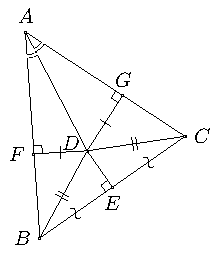
\includegraphics[width=35mm]{M67_2017-18_TD1_img1}
  }
\end{exo}


%-----------------------------------
\begin{exo} (Triangle isocèle)

  Soit $\tri ABC$ un triangle isocèle avec $AB=AC > BC$. On porte des points $D$ sur $(AB)$, avec $B$ entre $A$ et $D$, et $E$ sur $(BC)$, avec $C$ entre $B$ et $E$, et tels que $BD=CE=AB-BC$.

  Montrer que $\tri ADE$ est un triangle isocèle.
\end{exo}


% ==================================
\section{Nombres constructibles à la règle et au compas}
% ==================================


\begin{convention}\small
  Un point $M$ du plan est constructible en un pas (sous-entendu à la règle et au compas) à partir d'un ensemble de points $S=\{A_1,\ldots,A_k\}$ si c'est un point d'intersection
  \begin{itemize}
    \item de deux droites distinctes passant chacune par deux points de $S$,
    \item ou d'une droite passant par deux points distincts de $S$ et d'un cercle centré en un point de $S$ et passant par un autre point de $S$,
    \item ou de deux cercles distincts centrés en des points de $S$ et passant par des points de $S$.
  \end{itemize}

  Un point $M$ est dit \emph{constructible à partir de $S$} s'il est constructible en un nombre fini de pas, c'est à dire s'il existe $M_1,M_2,\ldots,M_{r-1},M_r=M$ tels que $M_{i+1}$ est constructible en un pas à partir de $S \cup \{M_1,\ldots,M_{i}\}$ pour tout $i=1,\ldots,r-1$.

  Un point \emph{constructible} est un point constructible à partir de $O=(0,0)$ et $I=(1,0)$.

  Enfin, un nombre réel $x$ est un \emph{nombre constructible} si le point $(x,0)$ est constructible. Plus généralement, un nombre complexe $z=x+iy$ avec $x,y \in \R$ est constructible si le point $(x,y)$ est constructible. En utilisant l'identification habituelle entre $\C$ et $\R^2$,  cela revient à dire que le point d'affixe $z$ est constructible.
\end{convention}


%-----------------------------------
\begin{exo} (Premières constructions)

  Tracer à la règle et au compas les figures suivantes:
  \begin{enumerate}
    \item le symétrique d'un point $A$ par rapport à un point $O$,
    \item le milieu d'un segment $[AB]$,
    \item la médiatrice d'un segment $[AB]$,
    \item la parallèle à une droite $(AB)$ passant par un point donné,
    \item la perpendiculaire à une droite $(AB)$ passant par un point donné (attention aux cas particuliers),
    \item le partage d'un segment en $n$ segments de même longueur,
    \item la bissectrice d'un angle $\widehat{BAC}$,
    \item le centre d'un cercle donné,
    \item le cercle de centre $A$ et de rayon $BC$ (ainsi on peut ajouter dans la définition de point constructible les cercles centrés en un point déjà construit et de rayon égal à la distance entre deux points déjà construit, ce qui revient à reporter l'écartement du compas).
  \end{enumerate}
\end{exo}


%-----------------------------------
\begin{exo}  (Comment dépasser les bords de la feuille)

  Soient $\Delta$ et $\Delta'$ deux droites qui se coupent en un point $O$ situé en dehors de la feuille.
  \begin{itemize}
    \item Soit $A$ un point situé sur la feuille. Tracer la droite $(OA)$.
    \item Tracer la bissectrice de l'angle formé par les deux droites (plus précisement de l'angle saillant formé par les demi-droites de la feuille).
  \end{itemize}

\end{exo}


%-----------------------------------
\begin{exo}  (Polygones réguliers)

  \begin{itemize}
    \item Construire à la règle et au compas un triangle équilatéral, un carré, un hexagone régulier, un octogone régulier.
    \item Construire un pentagone régulier.
    \begin{indication}
      On peut calculer la valeur de $\cos \frac{2\pi}{5}$ en décomposant $X^4+X^3+X^2+X+1$ en produit d'irréductibles dans $\R[X]$.
    \end{indication}
  \end{itemize}
\end{exo}


%-----------------------------------
\begin{exo} (Nombres constructibles)

  \begin{enumerate}
    \item Montrer qu'un point $(x,y)$ est constructible si et seulement si ses deux coordonnées $x$ et $y$ le sont.
    \item Montrer que tout point de $\Z^2$ est constructible.
    \item Montrer que $\sqrt{2}$ et $\sqrt{3}$ sont constructibles.
    \item Montrer que tout rationnel est constructible.
  \end{enumerate}
\end{exo}


%-----------------------------------
\begin{exo}  (Structure de l'ensemble des nombres constructibles)

  Soit $\ens K$ l'ensemble  des nombres réels constructibles.
  \begin{enumerate}
    \item Montrer que $\ens K$ est un corps.
    \item Montrer que la racine carrée $\sqrt{x}$ d'un réel $>0$ constructible est encore constructible.
  \end{enumerate}
\end{exo}


%-----------------------------------
\begin{exo} \label{caracterisation} (Une caractérisation des nombres constructibles)

  \begin{enumerate}
    \item Soit $K$ un sous-corps de $\R$ et $d \in K$ un nombre $>0$. Montrer que l'ensemble $K(\sqrt{d})$ défini par $K(\sqrt{d})=\{a+b\sqrt{d}, a, b \in K\}$ est un sous-corps de $\R$ qui contient $K$ et $\sqrt{d}$. C'est le plus petit sous-corps de $\R$ contenant $K$ et $\sqrt{d}$.
    \item Soit $M=(x,y)$ un point constructible en un pas à partir d'un ensemble $S=\{M_1,\ldots,M_n\}$. Soit $K$ un corps contenant les coordonnées des points $M_1,\ldots,M_n$. Alors il existe $d \in K$, $d>0$ tel que $x,y \in K(\sqrt{d})$.
    \item Montrer qu'un nombre réel $x$ est constructible si et seulement si il existe une suite $\Q=K_0 \subset K_1 \subset \cdots \subset K_n$ de sous-corps de $\R$ tels que pour tout $i=1,2,\ldots,n$ il existe $d_i \in K_{i-1}$ tel que $K_i=K_{i-1}(\sqrt{d_i})$ et $x \in K_n$.
  \end{enumerate}
\end{exo}


%-----------------------------------
\begin{exo}  (Une condition nécessaire de constructibilité)
  \begin{enumerate}
    \item Soient $K \subset L$ deux corps (on dit que $L$ est une \emph{extension} de $K$). Constater que $L$ est un espace vectoriel sur $K$. On note souvent $[L:K]$ la dimension de $L$ comme espace vectoriel sur $K$, appelée \emph{degré de l'extension $L/K$}. Montrer que si $K \subset L \subset M$ est une tour d'extensions de degrés finis, alors $[M:K]=[M:L][L:K]$.
    \item Soient $L/K$ une extension de degré $[L:K]$ fini et $x \in L$. Montrer que $x$ est racine d'un polynôme $X^d+a_1 X^{d-1} + \cdots + a_d$ à coefficients dans $K$ (on dit que $x$ est \emph{algébrique} sur $K$), puis qu'il existe un unique polynôme à coefficients dans $K$ unitaire de degré minimal annulant $x$ (appelé \textit{polynôme minimal}). Montrer que le degré de ce polynôme minimal (appelé \emph{degré} de $x$ sur $K$) divise $[L:K]$.
    \item En déduire, en utilisant \ref{caracterisation}, que si $x$ est un réel constructible, alors le degré de $x$ sur $\Q$ est une puissance de $2$.
  \end{enumerate}
\end{exo}


%-----------------------------------
\begin{exo}  (Résolution de quatre problèmes grecs)

  Les Grecs avaient laissé quatre problèmes de construction à la règle et au compas non résolus: \emph{quadrature du cercle}, \emph{duplication du cube}, \emph{trisection de l'angle} et \emph{construction des polygones réguliers}.

  La condition nécessaire précédente permet de montrer l'impossibilité de ces constructions.
  \begin{enumerate}
    \item (\emph{Quadrature du cercle}) Construire un carré de même aire qu'un disque donné.
    \begin{enumerate}
      \item Montrer que cela revient à construire le nombre $\sqrt{\pi}$.
      \item Le théorème de Lindemann assure que $\sqrt{\pi}$ est \emph{transcendant}, c.-à-d. non algébrique. En déduire que la quadrature du cercle est impossible.
    \end{enumerate}
    \item (\emph{Duplication du cube}) Partant d'un cube de volume donné, construire un cube de volume double.
    \begin{enumerate}
      \item Montrer que cela revient à construire le nombre $\sqrt[3]{2}$.
      \item Montrer que $\sqrt[3]{2}$ est un nombre algébrique et calculer son degré. Conclure.
    \end{enumerate}
    \item (\emph{Trisection de l'angle})  Partager un angle en trois angles égaux.
    \begin{enumerate}
      \item Montrer que trisecter l'angle $\frac{\pi}{3}$ revient à construire $\cos(\frac{\pi}{9})$.
      \item Montrer que $\cos 3\theta = 4 \cos^3 \theta -3 \cos \theta$. En déduire que $2 \cos \frac{\pi}{9}$ est racine du polynôme $P(X)=X^3-3X-1$.
      \item Montrer que $P$ n'a pas de racine dans $\Q$. Conclure.
    \end{enumerate}
    \item (\emph{Construction des polygones réguliers}) Construire le polygone régulier à $n$ côtés.
    \begin{enumerate}
      \item Montrer que construire l'heptagone régulier revient à construire $\cos\frac{2i\pi}{7}$.
      \item Notons $\zeta_7=e^{\frac{2i\pi}{7}}$. Montrer que $\zeta_7$ est racine du polynôme $X^6+X^5+X^4+X^3+X^2+X+1$.
      \item Montrer que, si $K$ est un sous-corps de $\R$ contenant $\cos\frac{2i\pi}{7}$, alors $\zeta_7$ appartient à $K(i\sqrt{d})$ pour un certain $d \in K$.
      \item En déduire que si $\cos\frac{2i\pi}{7}$ est constructible, alors $\zeta_7$ est de degré $2$ sur $\Q$. Conclure.
      %C'est dur: deja il y a une petite subtilite de redaction, on obtient d'abord que l'ordre de $\zeta_7$ divise 2, et ce n'est pas 1 car $\zeta_7$ n'est pas rationnel. Ensuite, on peut dire que le polynome minimal de $\zeta_7$ etant de degre 2, c'est $(X-\zeta_7)(X-\overline{\zeta_7})$, d'ou cos 2pi/7 rationnel.
    \end{enumerate}
  \end{enumerate}
\end{exo}


\end{document}
